\chapter{The LHCb detector at the Large Hadron Collider}
\label{sec:Detector}

\section{The Large Hadron Collider}

The Large Hadron Collider (LHC)~\cite{Evans:2009zzc} is a circular particle accelerator with a circumference of 27~km located about 100~m underground
in the surroundings of Geneva, Switzerland. Two proton beams circulate in opposite directions around the ring and cross each
other at several points, in which particle detectors are placed. These include two general-purpose detectors, ATLAS and CMS,
siting on opposites sides of the ring and the two smaller specialty detectors, ALICE and LHCb, are at the interaction points
to either side of ATLAS (see fig. \ref{lhc}).

\begin{figure}[h!]
\centering
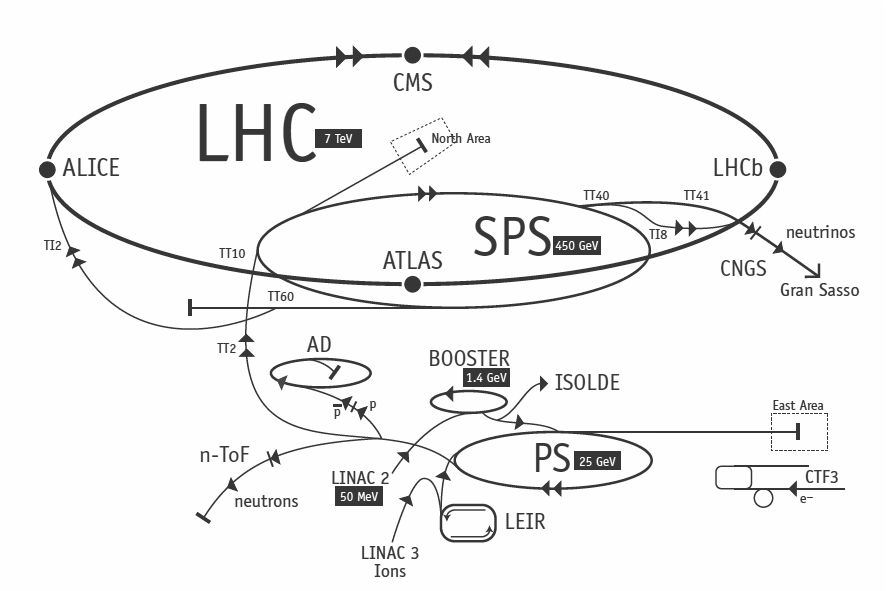
\includegraphics[width=1\textwidth]{Detector/figs/LHC_scheme.png}
\caption{Scheme of CERN accelerators.} \label{lhc}
\end{figure}

Each beam consists of a series of proton bunches, up to a maximum of 2835. Each bunch consists of about $10^{11}$
protons and the bunch spacing is such that the nominal bunch crossing rate is 40 MHz. The beams are injected into
pre-accelerators and then led into LHC through the CERN acceleration system shown in Fig.~\ref{lhc}. Protons are
produced from hydrogen gas and are initially accelerated to the energy of 50 MeV in a linear accelerator (LINAC).
Then they are injected into the Proton Synchrotron Booster (PSB), where they are boosted to an energy of 1.4 \gev,
into the Proton Synchrotron (PS) to 25 GeV and into the Super Proton Synchrotron (SPS) to 450 GeV. Finally, protons
enter into the LHC storage ring. In the main ring proton beams are accelerated from injection energy to the final one
by radio frequency (RF) cavities. The beams are steered around the ring by 8~T magnetic fields produced in 15~m long
superconducting niobium-titanium dipole magnets and focused by quadrupole and multipole magnets. The LHC magnets
use a design in which both proton beam pipes are contained in the same housing, allowing the same liquid helium to cool 
the system down for both. The LHC began colliding proton beams in physics mode in 2009 at a center of mass
energy of $\sqrt{s} = 900$ \gev and from April 2010 to November 2011 accelerated beams at $\sqrt{s} = 7$ \tev (3.5 \tev per
proton beam). At this energy it delivered over $5.7 \text{ fb}^{-1}$ of collisions, with a maximum instantaneous
luminosity of $3\cdot10^{33} \text{ cm}^{-2}\text{s}^{-1}$. The LHC maximum design energy is 14 TeV, and its design
luminosity is $10^{34} \text{ cm}^{-2}\text{s}^{-1}$. After a long shut down to upgrade and maintain the machine, a
new run started in June 2015 where protons are collided at a center of mass energy of $\sqrt{s} = 13$ \tev. At this
energy the total proton-proton cross section is expected to be roughly 100 mb.
%, thus at the design luminosity the general purpose detectors will an event rate approximately $10^9$ inelastic events/s.

\section{The LHCb detector}

The LHCb detector~\cite{Alves:2008zz} was built with the main purpose of studying the decays of B and D mesons, looking in particular for
CP-violating processes. In 2011, running at a centre of mass energy of 7 TeV, the cross section of $b\bar{b}$ production
was measured to be $284 \pm 53 ~\mu b$~\cite{Aaij:2010gn}, while it will be $\sim500 ~\mu b$ at the current LHC energy, 13 TeV.
At these high energies, proton-proton interactions produce highly boosted virtual gluons which interact to produce $b\bar{b}$
pairs at small angles, close to the beam pipe. For this reason the LHCb detector is designed to have a very forward angular
coverage: it is fully instrumented from approximately 10 mrad to 300 mrad, corresponding to $2 < \eta < 5$, where $\eta$
is the ``pseudorapidity", a quantity used in particle physics and called and defined as:
\begin{equation}
\label{pseudorap}
\eta = - \ln(\tan(\theta/2))
\end{equation}
In Eq.~\ref{pseudorap}, $\theta$ is the angle between a particle's momentum and the beam direction
\footnote{LHCb's reference system has the $z$ axis in the direction of the beam, the $x$ axis directed to
the centre of the accelerator and $y$ is directed upward. Then we define $\theta$ as the angle with the beam
direction and $\phi$ as the position around the beam in the $xy$ plane, taking $\phi = 0$ on the $x$ axis.}.

\begin{figure}[h]
\label{lhcb}
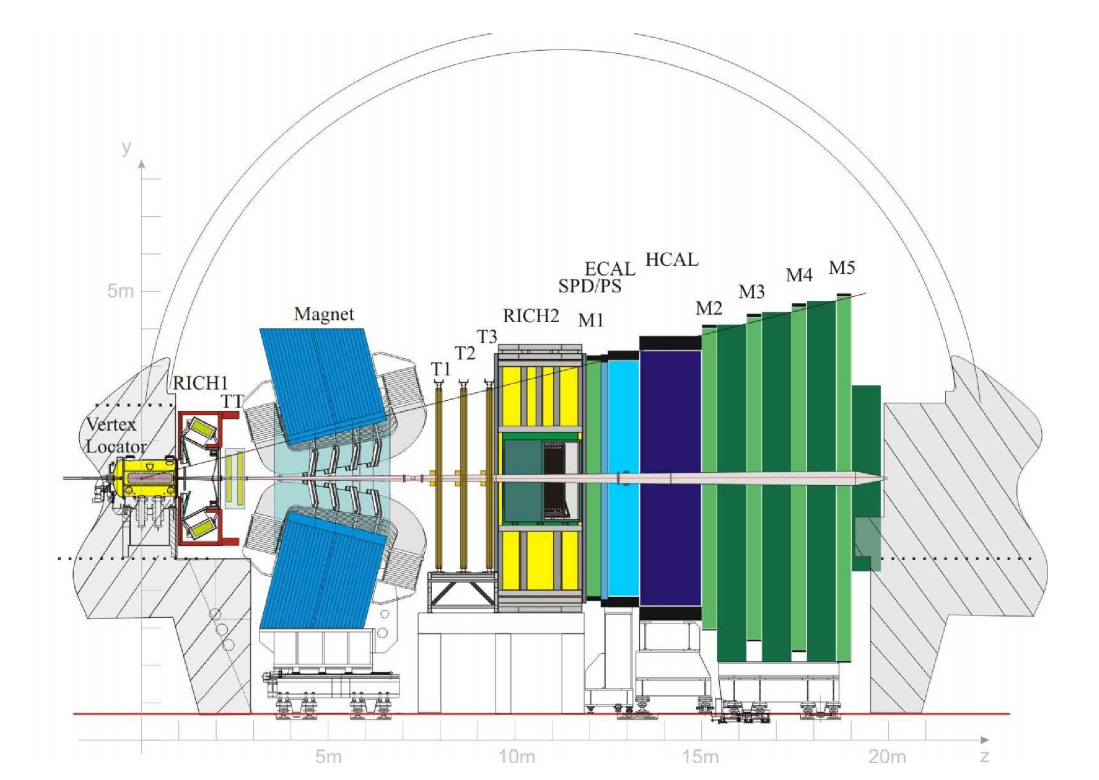
\includegraphics[width=0.95\linewidth]{Detector/figs/LHCb_official.png}
\caption{A side view of the LHCb detector~\cite{Alves:2008zz}.}
\end{figure}

At the collision point of LHCb the luminosity can be adjusted by displacing the beams from head on collisions
while keeping the same crossing angle. This allows the experiment to keep an approximately constant instantaneous
luminosity. This also means that the average number of interactions per bunch crossing can be limited as the detector
efficiency, especially in detecting secondary vertices, decreases for events with an high number of primary vertices (PV).
Reducing the particle occupancy through the detector also keeps radiation damage to a minimum. Since the LHC started colliding
protons in November 2009 until the end of 2011, the instantaneous luminosity was at an average of
$3 \cdot 10^{32} \mbox{cm}^{-2}\mbox{s}^{-1}$, with an average number of 1.5 vertices per bunch crossing in LHCb.
At the end of 2011 LHCb had collected an integrated luminosity of 1 \invfb; in 2012 the luminosity was increased
and 2 \invfb more were collected.

Other B physics experiments, like BaBar at the Stanford Linear Accelerator (SLAC), Belle at KEK at J-PARC (Japan)
and the Tevatron experiments at Fermilab have made accurate measurements in heavy flavour physics. All of these
results have so far been consistent with the Standard Model predictions. However, some of the deviations from the
Standard Model are expected to be very small, therefore LHCb has begun to make the most precise measurements
in heavy flavour physics to test the consistency of the Standard Model and look for new physics.

The LHCb detector includes a high-precision tracking system consisting of a silicon-strip
vertex detector surrounding the $pp$ interaction region, a large-area silicon-strip detector located upstream
of a dipole magnet with a bending power of about 4 Tm, and three stations of silicon-strip detectors and straw
drift tubes placed downstream. The combined tracking system has momentum resolution $\Delta p/p$, that varies
from 0.4\% at 5 $\mbox{GeV/c}^{2}$ to 0.6\% at 100 $\mbox{GeV/c}^{2}$. Charged hadrons are identified using two
Ring-Imaging Cherenkov detectors (RICH)~\cite{LHCb-DP-2012-003}. Photon, electron and hadron candidates are
identified by a calorimeter system consisting of scintillating-pad and pre-shower detectors, an electromagnetic
calorimeter and a hadronic calorimeter. Muons are identified by a system composed of alternating layers of iron
and multiwire proportional chambers~\cite{LHCb-DP-2012-002}. A schematic view of the detector is shown in Fig.~\ref{lhcb}
and more details on each subdetector are given in the following sections.

\section{The magnet}

Charged particle tracks are bent horizontally in the magnetic field
so that their momentum can be measured from the curvature radius.
The LHCb dipole magnet is comprised of two coils supported on an iron yoke
and is shaped to fit the LHCb angular acceptance. Unlike the other LHC experiments,
LHCb uses a warm magnet, so that it can be ramped easily and the field can be reversed periodically.
When the polarity is flipped and particles of a given sign are bent in the opposite direction. 
This is method is used used to limit systematic uncertainties that can arise form different performances
in different areas of the detector and average out using data taken in both polarities.
In the magnet flow a 5.85~kA current that generates an integrated magnetic field of 4~Tm for 10~m long tracks.
In order to achieve the required momentum precision the magnetic field must be mapped with
a $10^{-4}$ precision. For this reason a grid of 60 sensors is positioned inside the magnet
and provides real time magnetic field maps.

\section{Tracking system}

B mesons have lifetimes of approximately 1.5 ps. At the LHC energies, this means they travel about
1~cm before decaying and they form a displaced vertex. To study specific decays, it is therefore important
to be able to separate the particles produced at the primary $pp$ vertex and the B decay vertex.
The tracking system consists in the Vertex Locator (VeLo), and 4 tracking stations:
the Tracker Turicensis (TT), which are located before the magnet and the T1, T2 and T3 stations,
located downstream of the magnet. The latter tree stations are in turn formed by two subsystems:
the Inner Tracker (IT) close to the beam-line, where the particle density is greatest and
the Outer Tracker (OT) covering the rest of the acceptance.
%
\begin{center}
\begin{figure}[h!]
\centering 
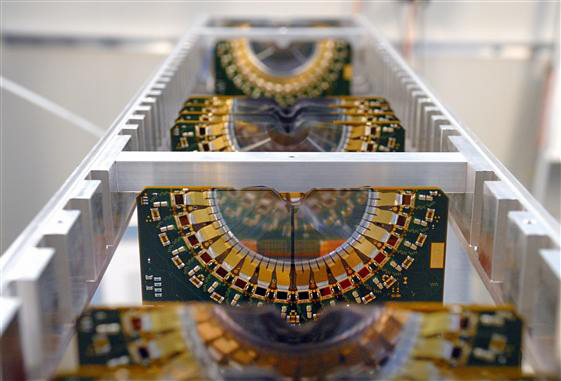
\includegraphics[width=0.49\textwidth]{Detector/figs/detector/VELO.png}
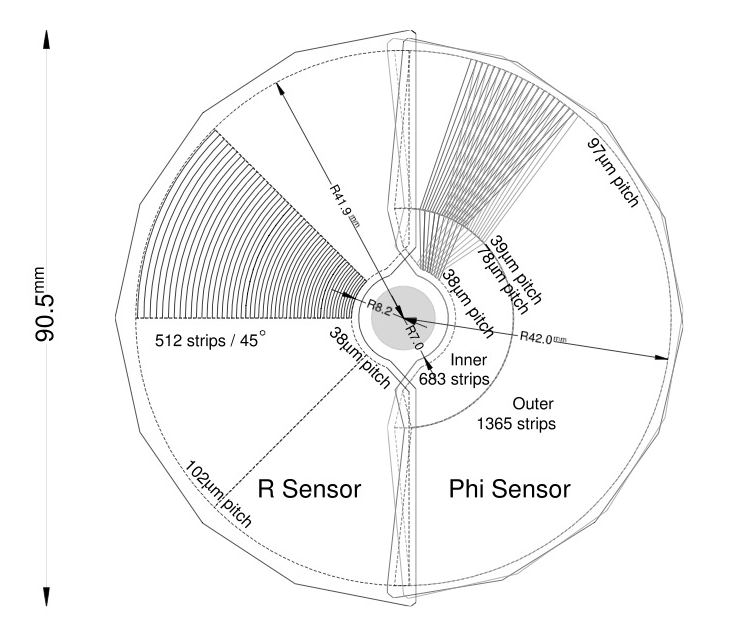
\includegraphics[width=0.49\textwidth]{Detector/figs/detector/VELO_scheme.png}
\caption{On the left VeLo sensors mounted in line and on the right a schematic view of one sensor~\cite{Alves:2008zz}.}
\label{VeLo}
\end{figure}
\end{center}
%
The VeLo accurately measures positions of tracks close to the interaction point so that production
and decay vertices of bottom and charm hadrons can be reconstructed. The VeLo is composed by 21 staggered
silicon modules which surround the beam axis and are positioned from $z = -18$~cm to $+80$~cm.
It is able to detect particles within a pseudorapidity range $1.6 < \eta < 4.9$. The sensitive region
of the VeLo starts at an inner diameter of only 8~mm from the beam axis. The VeLo is housed in its own
vacuum vessel of thin aluminium foil which protects the vacuum of the beam pipe from any outgassing of
the VeLo. The silicon layers composing the VeLo consist of two modules each including two types of sensors:
the $\phi$-sensor which measures the azimuthal position around the beam, and the R-sensor which measures
the radial distance from the beam axis. A sketch of the VeLo sensor is shown in Fig.~\ref{VeLo}. The sensors
are 300 $\mu m$ thick, approximately semicircular and are positioned on either side of the beam axis.
To ensure that they cover the full azimuthal angle the right-side module is placed 1.5~cm behind the left-side
module on the z-axis and they overlap. There are two modules which cover the backward direction
and are used as a veto for multiple interactions, this is called the pileup system.
%
\begin{center}
\begin{figure}[h!]
\centering 
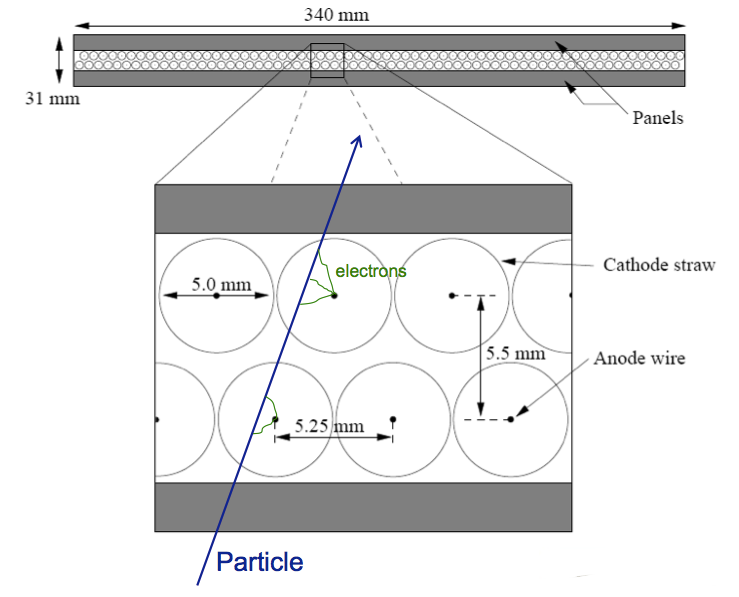
\includegraphics[width=0.8\textwidth]{Detector/figs/straw_tubes.png}
\caption{Sketch of the straw tubes which constitute the Outer Tracker layers~\cite{Alves:2008zz}.}
\label{fig:straw:tubes}
\end{figure}
\end{center}
%
The IT and TT both use silicon microstrips and together constitute the Silicon Tracker (ST). Straw tubes are used 
in the OT, of which a sketch is shown in Fig.\ref{fig:straw:tubes}. The IT requires an higher inner granularity
because of the higher flux of particles nearer the beam pipe, in fact it covers only 1.3\% of the total
are of IT plot OT but it contains about 20\% of the tracks. Each ST station has four detection layers,
the first and last being vertical, measuring the track position in x. The second 
and third layer are rotated by a stereo angle of +5 and -5 degrees, which allows the y-coordinate to be measured. 
The TT is placed upstream of the magnet, which allows reconstruction of the tracks from low-momentum particles
which are swept out of the downstream acceptance. Overall the tracking system provides a measurement of momentum, $p$, 
with a relative uncertainty that varies from 0.5\% at low momentum to 1.0\% at 200 \gevc. The impact parameter (IP),
namely the minimum distance of a track to a primary vertex, is measured with a resolution of $(15 + 29/\pt)$ $\mu m$,
where \pt is the component of the momentum transverse to the beam, in \gevc.


\section{Particle identification}

Particle identification is an important feature in LHCb and it is performed in various ways.
The electromagnetic calorimeters can distinguish between pions and electron, the muon chambers
identify muons and the Ring Imaging Cherenkov (RICH) detectors can be used to identify 
heavier charged particles as protons and kaons.

\subsection{Calorimeters}
\label{sec:calorimeters}

The main purpose of the calorimeter system is to determine the energy of particles traversing the detector. 
A calorimeter is composed by layers of absorber and active material. The absorber makes particles
interact and produces a cascade of secondaries, which multiply quickly and are detected by the active part.
In LHCb the sensitive material consists of scintillating layers, where the light detected is approximately proportional 
to the number of deposited particles. Calibration is then used to traslate the signal into a measurement of deposited
energy. 
%The calorimeter system is essential for flavour tagging because it identifies electrons. In addition, it
%is required for accurately reconstructing $\pi^0$ particles and prompt photons, which are both needed for the study of B-meson decays.
The LHCb calorimeter system consists of the Scintillator Pad Detector (SPD), the Pre-Shower Detector (PS) as well as
the Electromagnetic Calorimeter (ECAL) and the Hadronic Calorimeter (HCAL).
The most difficult identification is that of electrons. First of all the rejection of a high background
of charged pions requires a longitudinal segmentation of the electromagnetic calorimeters. This is provided by
the PS detector added in front of the main electromagnetic calorimeter, ECAL. Electrons also have to be 
distinguished from high energy $\pi^0$s. For this purposed the SPD calorimeter, detecting charged particles,
is located in front of the PS and ECAL detectors. Fig.~\ref{fig:pi0_e_pid_perf} shows how the ratio of the
energy detected in the ECAL and the particle momentum allows the separation of electrons and hadrons.
All four detectors transmit scintillation light via
wavelength-shifting fibres to photo-multiplier tubes (PMTs). The SPD/PS cells are read out with MAPMTs 
(Multi-anode PMTs) located outside the LHCb acceptance. Instead the ECAL and HCAL have individual MAPMTs
located on the modules. All four detectors are segmented, which allows to achieve to associate the energy
deposits to tracks in the tracking system. The segmentation of the cells vaies according to the distance from the beam pipe.
%The purpose of the SPD and PS is to separate the electrons from a high background of neutral and charged pions 
%produced in the collisions. 

\begin{figure}[t!]
\centering
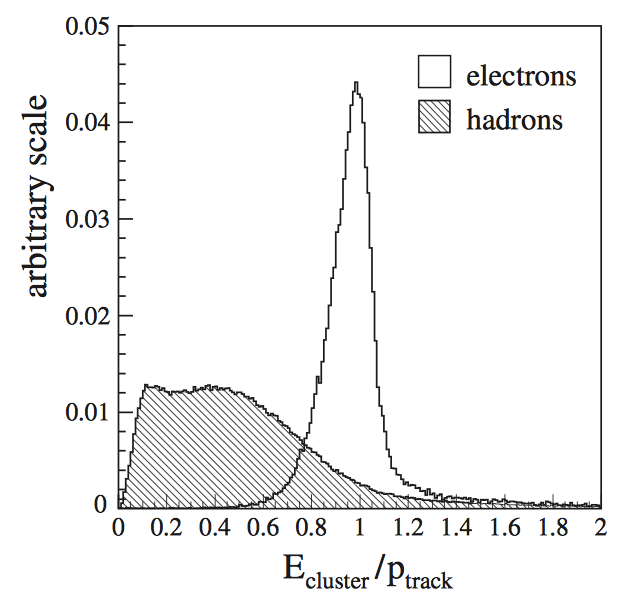
\includegraphics[width=0.5\textwidth]{Detector/figs/pi0_e_pid_perf.png}
\caption{The ratio of the energy deposited in the ECAL and the particle momentum, which allows
the separation between electrons and hadrons. }
\label{fig:pi0_e_pid_perf}
\end{figure}

In order to obtain the highest energy resolution the showers from high energy photons 
must be fully absorbed. For this reason the ECAL has a thickness of 25 radiation lengths and its resolution is 
measured to be~\cite{Alves:2008zz}
 %
 \begin{equation}
 \frac{\sigma_{ECAL}(E)}{E} = \frac{10\%}{\sqrt{E(GeV)}} + 1\%,
 \end{equation}
%
which results in a mass resolution of $\sim 70$ \mevcc or B mesons for $\sim 8$ \mevcc for \piz.
The trigger requirements on the HCAL resolution do not depend on the containment of the hadron showers as much 
as for the ECAL, so due to a limited space, its thickness is only 5.6 interaction lengths and its resolution
%
 \begin{equation}
 \frac{\sigma_{HCAL}(E)}{E} = \frac{69\%}{\sqrt{E(GeV)}} + 9\%.
 \end{equation}

\subsubsection{Breamsstrahlung recovery for electrons}

Bremsstrahlung is an electromagnetic radiation produced by particles, that decelerate or deviate because of
the presence other charged particles. Typically electrons produce Bremsstrahlung when deflected by atomic nuclei.
The probability of emitting breamsstrahlung radiation is proportional to the inverse of the squared mass of the
particle ($1/m^2$) and therefore is relevant only for electrons.
%
\begin{figure}[h!]
\label{bremreco}
\centering
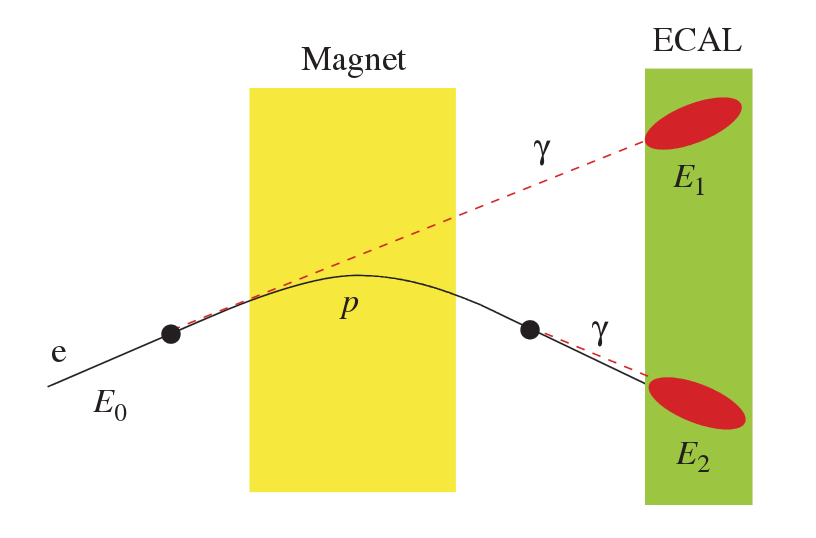
\includegraphics[width=0.55\textwidth]{RKst/figs/brem_recovery.png}
\caption{Schematic view of the Breamsstrahlung recovery. }
\end{figure}
%
At these energies, if electrons radiate after
the magnet, the photon will hit in the same calorimeter cells as the electron and the energy will be automatically
recovered. However, if the photon is emitted before the magnet, the electron will be deflected by the magnetic
field whereas the photon will continue on its initial trajectory, with its energy being deposited in a different
part of the calorimeter. Missing this energy results in a poorer reconstructed \Bz mass resolution, so it is
desirable to recover these bremsstrahlung photons, when possible. A tool for bremsstrahlung recovery is available
in the LHCb analysis software. This tool looks for other clusters in the calorimeter and reconstructing the trajectory
of the electron checks if they may have been emitted by that. Then the photon energy is added to the electron and its
momentum recalculated. Figure~\ref{bremreco} shows a schematic view of the process. For more information see
Ref.~\cite{LHCb:2003ab}.

\subsection{RICH}

The two RICH detectors are a special feature of LHCb, as it is the only experiment at LHC including them. 
These detectors take advantage of the Cherenkov radiation produced by particles passing in a medium with velocity 
higher than the velocity of light in the medium. The Cherenkov light, as shown in Fig.~\ref{Cherenkov}, 
is produced in cones with a specific angle depending on the velocity of the particle. The relation
between the angle and the particle velocity can be written as 
%
\begin{equation}
cos(\theta) = \frac{1}{\beta n}
\end{equation}
%
where $\beta$ is the particle velocity over $c$ and $n$ is the refraction index of the medium.
%
\begin{figure}[h!]
\centering
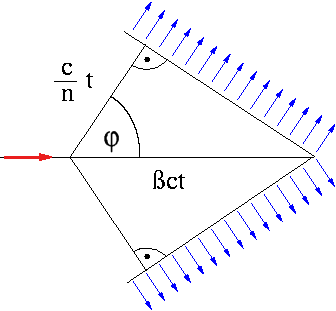
\includegraphics[width=0.45\textwidth,height=5.5cm]{Detector/figs/detector/Cherenkov.png}
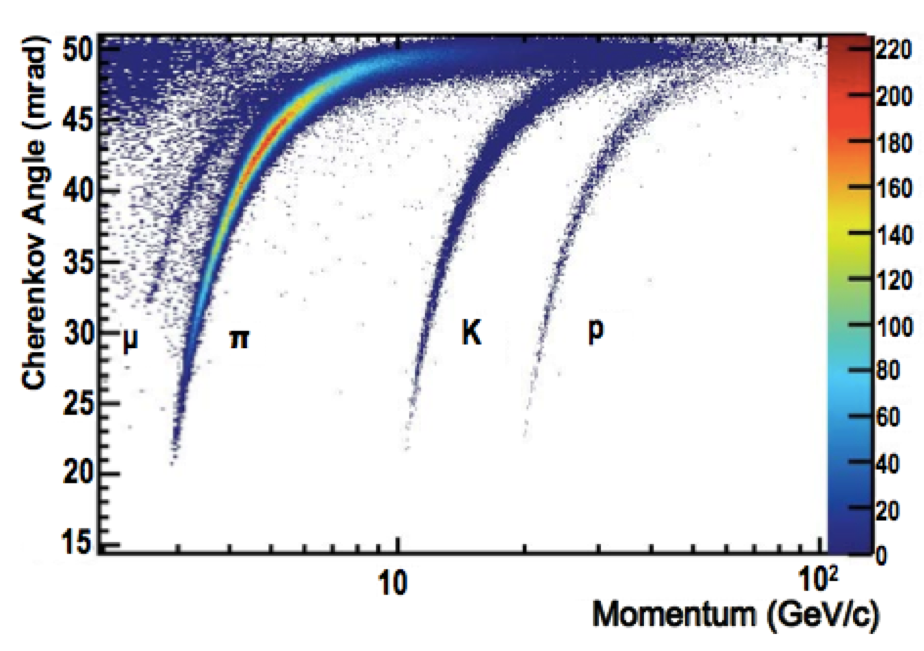
\includegraphics[width=0.45\textwidth,height=5.5cm]{Detector/figs/changle_vs_momentum.png}
\caption{On the left a sketch of Cherenkov light emission and on the right the Cherenkov
angle versus momentum for the two radiators of RICH1 and for different particles. One can see that they allow
to separate particles in different momentum ranges.}
\label{Cherenkov}
\end{figure}

RICH 1 is situated before the magnet in order to cover a large angular acceptance. Its purpose is to ensure
particle identification over the momentum range $1 < p < 70$ \gevc. It uses two radiators: $C_4F_{10}$ that covers
the momentum range $5 - 70$ \gevc and silica aerogel which covers $1 - 10$ \gevc. RICH 2 is positioned after
the magnet and tracking stations. It identifies higher momentum particles from approximately 20 \gevc up to beyond
100 \gevc using $CF_4$ as a radiator.
The Cherenkov light produced when charged particles travel through the radiators, is reflected and focused using
flat and spherical mirrors, which are tilted so that the ring image is reflected onto arrays of photo-detectors.
The radius of the ring can be used to measure the opening angle of the Cherenkov cone because of the known geometry.
The photo-detectors are located outside of the LHCb acceptance in order to reduce the amount of material that
the particles have to traverse. Pattern recognition algorithms are then used to reconstruct the Cherenkov rings.

%For particle identification a particle type hypothesis is assigned to each charged track found in the tracking stations.
%Initially the hypothesis is for a pion, which is the most common particle type. The corresponding expected number and
%Cherenkov radii of the resulting photons are calculated and the likelihood is calculated. The hypothesis is then changed
%and the likelihood is recalculated. The case with the largest increase in likelihood is kept.


\section{The muon system}

It is essential for many of the key physics analyses to be able to identify muons in the final state.
Muons are the most penetrating particles that can be detected at LHC experiments, so the muon chambers
are the farthest subdetectors from the interaction point. The muon system is formed by five stations (M1 - M5),
the first one being located before the calorimeters in order to improve \pt measurements. A scheme of the muon
system is shown in Fig.~\ref{muonsystem}. The remaining four stations lay behind the HCAL and are separated by 1.2~m
from each other, interleaved with iron 80~cm thick blocks, which absorb hadrons, electrons and photons to ensure
that only muons reach the final muon station. Only muons with a minimum momentum of 10 \gevc traverse all of the
five stations and for positive identification of a muon the trigger requires a signal in each of them.
Each station has a detection efficiency of at least 95\% and the detectors provide position measurements.
Since there is a larger particle flux towards the beam pipe, the stations are divided
into four concentric rectangular regions (R1-R4), their size increasing according to the ratio 1 : 2 : 4 : 8.
This results in a similar channel occupancy over the four regions. All of the muon stations use
Multi Wire Proportional Chambers (MWPC) except for the inner region of M1, where the particle flux is too high.
In this region triple-GEM (Gas Electron Multiplier) detectors are used because of their better ageing properties.
%
The Gas Electron Multiplier (GEM) detectors in the inner region of M1 have to withstand a rate up to
$500 ~\mbox{kHz cm}^{-2}$ of charged particles. In these detectors particles traversing through the drift gap
between the cathode and the first GEM foil produce ionisation electrons, which are then attracted by electric fields
though all of the GEM foils and multiply. They then drift into the anode inducing a signal on the pads. A gas mixture
of Argon, $CO_2$ and $CF_4$, is used to give a time resolution better than 3~ns.
%
\begin{figure}[h!]
\label{muonsystem}
\centering 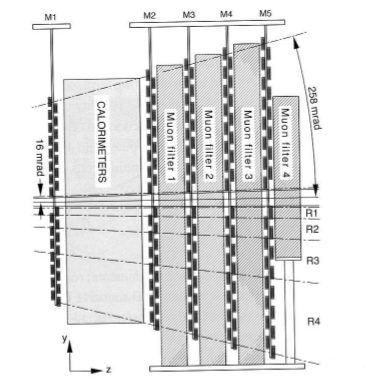
\includegraphics[width=0.65\linewidth]{Detector/figs/muonsystem.png}
\caption{The LHCb muon system~\cite{Alves:2008zz}.}
\end{figure}



\section{Trigger and software}

The LHCb trigger system~\cite{LHCb-DP-2012-004} consists of a hardware stage (L0), based on information from the calorimeters
and muon system, followed by a software stage, the High-Level Trigger (HLT), which applies a full event reconstruction.
To increase performances the HLT is split again into stages (HLT1 and HLT2). The HLT1 phase happens in real time and saves
data in local disks while the HLT2 phases uses the resources available during periods with no beam. The event selected by
the HLT2 stage are then saved for offline analysis. The bunch crossing frequency is 40~$\mbox{MHz}$, which corresponds to
an instantaneous luminosity of $2 \cdot 10^{32} ~\mbox{cm}^{-2} \mbox{s}^{-1}$ for LHCb. About 15\% of the total number of
$\bquark\bquarkbar$ pairs produced will contain at least one $B$ meson with all of its decay products within the detector acceptance. This rate needs to be
reduced down to about 2~kHz so that the events can be written to disk. Fig.~\ref{triggerscheme}
shows a scheme of the trigger system.

\begin{figure}[h!]
\centering 
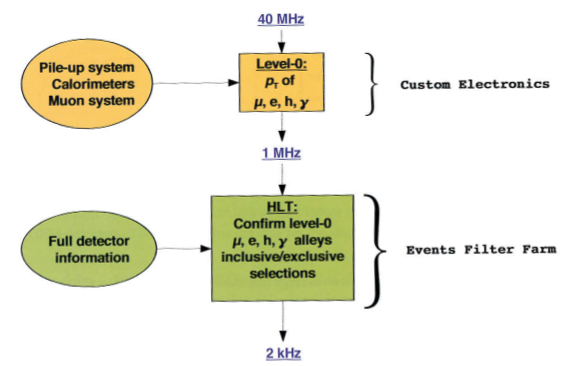
\includegraphics[width=0.9\linewidth]{Detector/figs/triggerscheme.png}
\caption{Scheme of the LHCb trigger system~\cite{Alves:2008zz}.}
\label{triggerscheme}
\end{figure}

The L0 trigger reduces the rate of visible interactions from 10~MHz to 1~MHz.
Due to the heavy mass of $B$ mesons, they often produce particles with high \pt or $E_{\rm T}$.
Therefore the trigger selects events with large $E_{\rm T}$ deposits in the calorimeter
of high \pt muons. The events is classified as \verb!L0Muon! it was triggered due to information
for the muon detector, while the information from the calorimeters is combined to divide the
events in the 5 categories: \verb!L0Photon!, \verb!L0Electron!, \verb!L0LocalPion!, \verb!L0GlobalPio!n, \verb!L0Hadron!. 
The label ``local" refers to $\pi^0$ reconstructed though their $\gamma\gamma$ decay, where the two photons
fall in the same ECAL element, they are labelled ``global" otherwise.
The HLT1 uses information from the VELO and trackers performing a partial reconstruction
of the event and reduces the rate to 2~kHz. Finally, the HLT2 involves a full reconstruction of the
event and includes many ``lines" designed to trigger specific decays.

LHCb also developed an extended simulation software in order to reconstruct efficiencies and signal shapes.
In the simulation, $pp$ collisions are generated using $\textsc{Pythia}8$~\cite{Sjostrand:2006za} with a specific
LHCb configuration~\cite{LHCb-PROC-2010-056}. Decays of hadronic particles are described by $\textsc{EvtGen}$~\cite{Lange:2001uf},
and final state radiation is generated using $\textsc{Photos}$~\cite{Golonka:2005pn}. Finally, the interaction of the generated
particles with the detector and its response are implemented using the $\textsc{Geant4}$ toolkit~\cite{Allison:2006ve}
as described in Ref.~\cite{LHCb-PROC-2011-006}. For this analysis in this thesis, the ROOT framework~\cite{Brun:2000es} was
used to analyse data and the RooFit package to perform maximum likelihood fits. A multivariate analysis is also used
based on the NeuroBayes package~\cite{Feindt:2006pm,feindt-2004} which provides a framework for neural network training.







